\documentclass[xetex,mathserif,serif]{beamer}
\usepackage{polyglossia}
\setdefaultlanguage[babelshorthands=true]{russian}
\usepackage{minted}
\usepackage{tabu}

\useoutertheme{infolines}

\usepackage{fontspec}
\setmainfont{FreeSans}
\newfontfamily{\russianfonttt}{FreeSans}

\definecolor{links}{HTML}{2A1B81}
\hypersetup{colorlinks,linkcolor=,urlcolor=links}

\tabulinesep=0.7mm

\title{Практика 1: Введение, потоки}
\author[Юрий Литвинов]{Юрий Литвинов \newline \textcolor{gray}{\small\texttt{yurii.litvinov@gmail.com}}}

\date{16.02.2018г}

\begin{document}
	
	\frame{\titlepage}

	\begin{frame}
		\frametitle{Правила игры}
		\begin{itemize}
			\item Пара один раз в две недели
			\begin{itemize}
				\item $=>$ вдвое больше домашки за один раз
			\end{itemize}
			\item Как обычно, куча домашек, две контрольные (и переписывание в конце), баллы и дедлайны, HwProj
			\begin{itemize}
				\item Задач будет немного меньше, но они немного объёмнее
			\end{itemize}
			\item За практику будет выставляться оценка, которая потом будет учитываться при сдаче экзамена
			\begin{itemize}
				\item по какой-то хитрой формуле, учитывающей баллы за домашку и контрольные
				\item \textcolor{gray}{Максимальный итоговый балл: 1.5, складывается из балла за контрольные (макс. 0.75) и балла за домашки (макс. 0.75). Максимум за к/р --- 16 баллов, максимум за д/з пока не известен}
			\end{itemize}
			\item Будет про многопоточные, сетевые, сетевые И многопоточные приложения, пользовательский интерфейс и т.д.
		\end{itemize}
	\end{frame}

	\begin{frame}
		\frametitle{Напоминание про штрафы}
		\begin{scriptsize}
			\begin{tabu} {| X[1 l p] | X[0.3 l p] |}
				\tabucline-
				\everyrow{\tabucline-}
				Пропущенный дедлайн                                                                   & баллы делятся на два \\
				Задача на момент дедлайна не реализует все требования условия                         & пропорционально объёму невыполненных требований \\
				Неумение пользоваться гитом                                                           & -2 \\
				Проблемы со сборкой (в том числе, забытый org.jetbrains.annotations)                  & -2 \\
				Отсутствие JavaDoc-ов для всех классов, интерфейсов и паблик-методов                  & -2 \\
				Отсутствие описания метода в целом                                                    & -1 \\
				Слишком широкие области видимости для полей                                           & -2 \\
				if (...) return true; else return false;                                              & -2 \\
				Именование классов-полей-методов-... и прочие code convertions                        & -1 \\
				Неиспользование try-with-resources там, где это было бы уместно                       & -1 \\
				Комментарии для параметров с заглавной буквы                                          & -0.5 \\
			\end{tabu}
		\end{scriptsize}
		\begin{center}
			\scriptsize{Список может расширяться!}
		\end{center}
	\end{frame}

	\begin{frame}
		\frametitle{Многопоточное программирование вообще}
		\begin{itemize}
			\item Плюсы
			\begin{itemize}
				\item Не вешать пользовательский интерфейс
				\item Равномерно распределять вычислительно сложные задачи по ядрам
				\item Выполнять одновременно несколько блокирующих операций ввода-вывода
			\end{itemize}
			\item Минусы
			\begin{itemize}
				\item Тысяча способов прострелить себе ногу
				\item Не всегда многопоточная программа работает быстрее однопоточной
			\end{itemize}
		\end{itemize}
	\end{frame}

	\begin{frame}
		\frametitle{Race condition}
		\begin{center}
			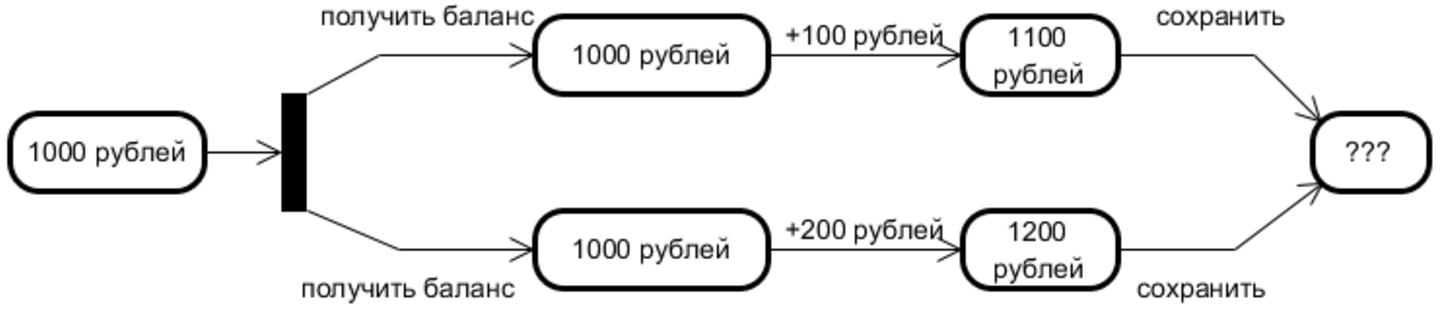
\includegraphics[width=0.9\textwidth]{raceCondition.png}
		\end{center}
	\end{frame}

	\begin{frame}[fragile]
		\frametitle{Маленький пример на race condition}
		\begin{footnotesize}
			\begin{minted}{java}
int[] a = new int[1000];
for (int i = 0; i < a.length; ++i) {
    a[i] = 1;
}

int[] result = new int[1];

for (int i = 0; i < 100; ++i) {
    final int localI = i;
    new Thread(() -> {
        for (int j = localI * 10; j <= (localI + 1) * 10 - 1; ++j) {
            result[0] += a[j];
        }
    }).start();
}

Thread.sleep(100);

System.out.println("Result = " + result[0]);
			\end{minted}
		\end{footnotesize}
	\end{frame}

	\begin{frame}
		\frametitle{Deadlock}
		\begin{center}
			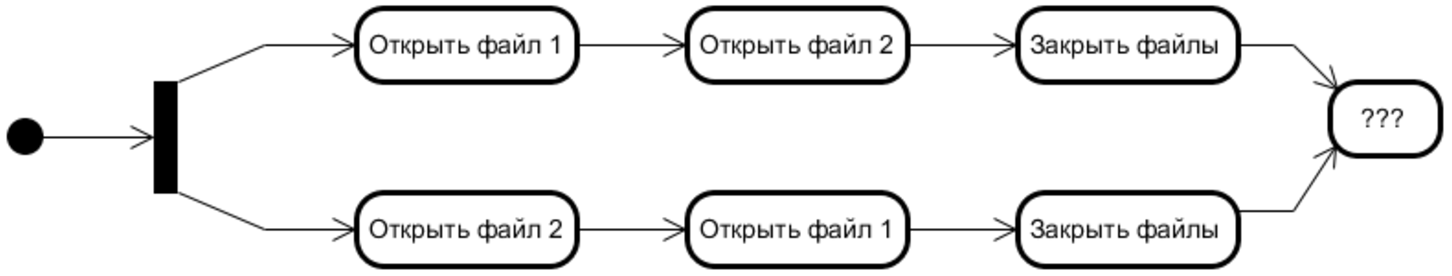
\includegraphics[width=0.9\textwidth]{deadlock.png}
		\end{center}
	\end{frame}

	\begin{frame}[fragile]
		\frametitle{Очень маленький пример на deadlock}
		\begin{footnotesize}
			\begin{minted}{java}
Thread.currentThread().join();
			\end{minted}
		\end{footnotesize}
	\end{frame}

	\begin{frame}
		\frametitle{Пример, потоки в Windows}
		\begin{itemize}
			\item Thread Kernel Object (\textasciitilde1240 байт)
			\item Thread environment block (TEB) (4 Кб)
			\item User-mode stack (1 Мб)
			\item Kernel-mode stack (24 Кб)
		\end{itemize}

		Ещё для каждой dll-ки, загруженной для процесса при старте или остановке потока вызывается DllMain с параметрами DLL\_THREAD\_ATTACH и DLL\_THREAD\_DETACH

		\vspace{3mm}
		Квант времени --- ~20-30 мс, после чего происходит \textit{переключение контекстов}
	\end{frame}

	\begin{frame}
		\frametitle{Как делать не надо}
		\begin{center}
			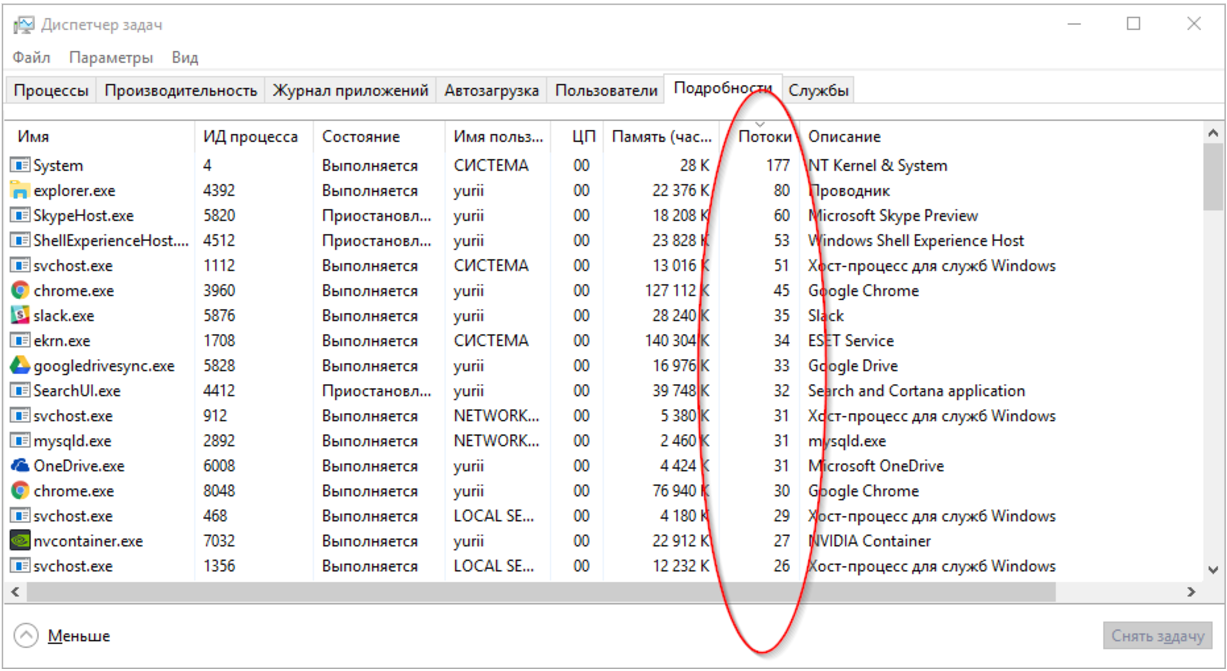
\includegraphics[width=0.9\textwidth]{threadsEverywhere.png}
		\end{center}
	\end{frame}

	\begin{frame}
		\frametitle{Задача на дом (пул потоков)}
		\begin{itemize}
			\item Нужно реализовать простой пул задач с фиксированным числом потоков (число задается в конструкторе)
			\item При создании объекта ThreadPoolImpl в нем должно начать работу n потоков
			\item У каждого потока есть два состояния: ожидание задачи и выполнение задачи
			\item Задача --- вычисление некоторого значения, вызов get у объекта типа Supplier<R>
			\item При добавлении задачи, если в пуле есть ожидающий поток, то он должен приступить к ее исполнению. 
					Иначе задача будет ожидать исполнения, пока не освободится какой-нибудь поток
			\item Задачи, принятые к исполнению, представлены в виде объектов интерфейса LightFuture
			\item Метод shutdown должен завершить работу потоков (через Thread.interrupt())
		\end{itemize}
	\end{frame}

	\begin{frame}
		\frametitle{LightFuture}
		\begin{itemize}
			\item Метод isReady возвращает true, если задача выполнена
			\item Метод get возвращает результат выполнения задачи
			\begin{itemize}
				\item В случае, если соответствующий задаче supplier завершился с исключением, этот метод должен завершиться с исключением LightExecutionException
				\item Если результат еще не вычислен, метод ожидает его и возвращает полученное значение
			\end{itemize}
		\end{itemize}
	\end{frame}

	\begin{frame}
		\frametitle{LightFuture}
		\begin{itemize}
			\item Метод thenApply --- принимает объект типа Function, который может быть применен к результату данной задачи X и возвращает новую задачу Y, принятую к исполнению
			\begin{itemize}
				\item Новая задача будет исполнена не ранее, чем завершится исходная
				\item В качестве аргумента объекту Function будет передан результат исходной задачи, и все Y должны исполняться на общих основаниях (т.е. должны разделяться между потоками пула)
				\item Метод thenApply может быть вызван несколько раз
				\item Метод thenApply не должен блокировать работу потока, если результат задачи X ещё не вычислен
			\end{itemize}
		\end{itemize}
	\end{frame}

	\begin{frame}[fragile]
		\frametitle{Примеры использования}
		\begin{footnotesize}
			\begin{minted}{java}
ThreadPoolmpl<Integer> pool = new ThreadPoolmpl<>(5);
LightFuture<Integer> task = pool.addTask(() -> 2 * 2);
assertThat(task.get(), is(4));

LightFuture<Integer> task1 = pool.addTask(() -> 2 * 3);
LightFuture<Integer> task2 = task1.thenApply((i) -> i + 1);
LightFuture<Integer> task3 = task1.thenApply((i) -> i + 2);
assertThat(task1.get(), is(6));
assertThat(task2.get(), is(7));
assertThat(task3.get(), is(8));
			\end{minted}
		\end{footnotesize}
	\end{frame}

	\begin{frame}
		\frametitle{Примечания}
		\begin{itemize}
			\item В данной работе запрещено использование содержимого пакета java.util.concurrent
			\item Все интерфейсные методы должны быть потокобезопасны
			\item Для каждого базового сценария использования должен быть написан несложный тест
			\item Обязателен билд в CI, на котором проходят ваши тесты
			\item Дедлайн: до \textbf{10:00 09.03.2018}
		\end{itemize}
	\end{frame}

	\begin{frame}[fragile]
		\frametitle{Задача на пару, многопоточный Lazy}
		Реализовать следующий интерфейс, представляющий ленивое вычисление:
		
		\begin{minted}{java}
public interface Lazy<T> {
  T get();
}
		\end{minted}

		\begin{itemize}
			\item Объект \textit{Lazy} создаётся на основе вычисления (представляемого объектом \textit{Supplier})
			\item Первый вызов \textit{get()} вызывает вычисление и возвращает результат
			\item Повторные вызовы \textit{get()} возвращают \textbf{тот же} объект, что и первый вызов
			\item Вычисление должно запускаться не более одного раза
		\end{itemize}
	\end{frame}

	\begin{frame}
		\frametitle{LazyFactory}
		Создавать объекты надо не вручную, а с помощью класса \textit{LazyFactory}, который должен
		иметь два метода с сигнатурами вида \textit{public static <T> Lazy<T> 
		create...Lazy(Supplier<T>)}, возвращающих две разные реализации \textit{Lazy<T>}:
		\begin{itemize}
			\item Простая версия с гарантией корректной работы в однопоточном режиме 
				(без синхронизации)
			\item Гарантия корректной работы в многопоточном режиме; вычисление не должно
				производиться более одного раза
			\begin{itemize}
				\item Что-то наподобие многопоточного синглтона
			\end{itemize}
		\end{itemize}
	\end{frame}
	
	\begin{frame}
		\frametitle{При этом}
		\begin{itemize}
			\item Ограничение по памяти на каждый \textit{Lazy}-объект: не больше двух ссылок
			\item \textit{Supplier.get} вправе вернуть \textit{null}
			\item Тесты
			\begin{itemize}
				\item Однопоточные, на разные хорошие и плохие случаи
				\item Многопоточные, на наличие гонок
			\end{itemize}
			\item Доделать дома
		\end{itemize}
	\end{frame}

\end{document}
